\documentclass[a4paper]{article}

% Formatting
\usepackage[utf8]{inputenc}
\usepackage[margin=1in]{geometry}
\usepackage[titletoc,title]{appendix}

% Math
% https://www.overleaf.com/learn/latex/Mathematical_expressions
% https://en.wikibooks.org/wiki/LaTeX/Mathematics
\usepackage{amsmath,amsfonts,amssymb,mathtools}

% Images
% https://www.overleaf.com/learn/latex/Inserting_Images
% https://en.wikibooks.org/wiki/LaTeX/Floats,_Figures_and_Captions
\usepackage{graphicx,float,subfigure}

% Tables
% https://www.overleaf.com/learn/latex/Tables
% https://en.wikibooks.org/wiki/LaTeX/Tables

% Algorithms
% https://www.overleaf.com/learn/latex/algorithms
% https://en.wikibooks.org/wiki/LaTeX/Algorithms
\usepackage[ruled,vlined]{algorithm2e}
\usepackage{algorithmic}
\usepackage{listings}

\usepackage[colorinlistoftodos]{todonotes}

\usepackage{xcolor}
\usepackage{listings}

\definecolor{mGreen}{rgb}{0,0.6,0}
\definecolor{mGray}{rgb}{0.5,0.5,0.5}
\definecolor{mPurple}{rgb}{0.58,0,0.82}
\definecolor{backgroundColour}{rgb}{0.95,0.95,0.92}

\lstdefinestyle{CStyle}{
    backgroundcolor=\color{backgroundColour},   
    commentstyle=\color{mGreen},
    keywordstyle=\color{magenta},
    numberstyle=\tiny\color{mGray},
    stringstyle=\color{mPurple},
    basicstyle=\footnotesize,
    breakatwhitespace=false,         
    breaklines=true,                 
    captionpos=b,                    
    keepspaces=true,                 
    numbers=left,                    
    numbersep=5pt,                  
    showspaces=false,                
    showstringspaces=false,
    showtabs=false,                  
    tabsize=2,
    language=C
}

\colorlet{keyword}{blue!100!black!80}
\colorlet{comment}{green!90!black!90}
\colorlet{STD}{blue!60!red!90}
\lstdefinelanguage{VHDL}{
   morekeywords=[1]{
     library,use,all,entity,is,port,in,out,end,architecture,of,
     begin,and, LIBRARY, USE, ALL, ENTITY, IS, PORT, IN, OUT, END, ARCHITECTURE, OF, BEGIN, AND
   },
   morekeywords=[2]{
     STD_LOGIC_VECTOR,STD_LOGIC,IEEE,STD_LOGIC_1164,
     NUMERIC_STD,STD_LOGIC_ARITH,STD_LOGIC_UNSIGNED,std_logic_vector,
     std_logic, downto, DOWNTO
   },
   morecomment=[l]--
}
\lstdefinestyle{vhdl}{
    language = VHDL,
    breakatwhitespace = false,         
    breaklines = true,                 
    captionpos = b,                    
    keepspaces = true,                 
    numbers = left,                    
    numbersep = 5pt,                  
    showspaces = false,                
    showstringspaces = false,
    showtabs = false,                  
    tabsize = 2,
    numberstyle =\tiny\color{mGray},
    basicstyle = \footnotesize,
    keywordstyle = [1]\color{keyword}\bfseries,
    keywordstyle = [2]\color{STD}\bfseries,
    commentstyle = \color{comment}
}


% Title content
\title{EN224 - Test et vérification}

\author{ALBERTY Maxime}
\date{9 février 2021}

\begin{document}

\maketitle

\tableofcontents

\newpage %-------Saut de Page---------

\section{Introduction}
    Ce TP à pour but de découvrir différentes méthodes de test et vérification dans le développement de composants logiciels et matériels.
\section{Software}
    \subsection{Etape 1}
        L'implémentation de la fonction PGCD fût une simple traduction de l'algorithme présenté en langage C.
\begin{lstlisting}[style=CStyle]
int PGCD(int A, int B)
{
	while(A != B){
		if (A > B){
			A = A - B;
		} else {
			B = B - A;
		}
	}
	return A;
}
 \end{lstlisting}
        
        Cependant il est important de resté concentré, car même si l'algorithme est trivial, une étourderie est vite arrivé et peut faire perdre du temps inutilement.
        \\
        
        Le test de la fonction est effectué au moyen de couples de valeurs d'on aura préalablement calculé le PGCD. 
\begin{lstlisting}[style=CStyle]
printf("PGCD(1024,800) = %d\n",PGCD(1024,800));
printf("PGCD(800,1024) = %d\n",PGCD(800,1024));
printf("PGCD(32767,65535) = %d\n",PGCD(32767,65535));
printf("PGCD(65535,32767) = %d\n",PGCD(65535,32767));
printf("PGCD(512,2048) = %d\n",PGCD(512,2048));
printf("PGCD(2048,512) = %d\n",PGCD(2048,512));
printf("PGCD(458,6272) = %d\n",PGCD(458,6272));
printf("PGCD(6272,458) = %d\n",PGCD(6272,458));
printf("PGCD(783,125) = %d\n",PGCD(783,125));
printf("PGCD(125,783) = %d\n",PGCD(125,783));
\end{lstlisting}
        Il faut ensuite comparé manuellement les résultats aux calculs.
        
        
    \subsection{Etape 2}
        Afin de pouvoir test plus de valeurs sans avoir à dupliquer les lignes de tests, nous ajoutons une génération aléatoires des valeurs de A et B comprisent entre 0 et 65535.
        
\begin{lstlisting}[style=CStyle]
#define MAX_RAND 65535
#define MIN_RAND 0 

int RandA(void){
	int A = (rand() % (MAX_RAND + 1 - MIN_RAND)) + MIN_RAND;
    return A;
}

int RandB(void){
	int B = (rand() % (MAX_RAND + 1 - MIN_RAND)) + MIN_RAND;
    return B;
}
\end{lstlisting}
        En ajoutant une boncle FOR dans le main, on peut ainsi test beaucoup plus de valeurs.
\begin{lstlisting}[style=CStyle]
for(int i = 0 ; i < 200000 ; i++){
	A = RandA();
	B = RandB();
	printf("%d\t%d\t%d\t%d\n", i, A, B,PGCD(A, B));
}
\end{lstlisting}
        
        \newpage
        Avec l'ajout de cette fonctionnalité, j'ai pu remarqué que la fonction PGCD ne prenait pas en compte les cas où $A = 0$ ou $B = 0$.
        Conformément à l'annexe du sujet, la fonction PGCD devient alors :
\begin{lstlisting}[style=CStyle]
int PGCD(int A, int B)
{
	while(A != B){
		if (A==0) return B; 
		if (B==0) return A;
		if (A > B){
			A = A - B;
		} else {
			B = B - A;
		}
	}
	return A;
}
\end{lstlisting}
        La vérification des résultats de la fonction PGCD est possible mais beaucoup trop long car il est nécessaire de comparer manuellement les résultats avec les calculs préalablement effectués.
    
    \subsection{Etape 3}
        Afin de tester plus de couple d'entrée, il peut être interressant de comparer ma fonction PGCD avec une autre déjà éprouver.
        La nouvelle approche est la suivante :
        \begin{itemize}
            \item Assignez à $N_1$ la valeur de $N_2$ et à $N_2$ la valeur du reste de la division de $N_1$ par $N_2$;
            \item Recommencez jusqu'à ce que le reste de la division soit nul;
            \item A ce moment, $N_1$ contient alors le PGCD de $N_1$ et $N_2$.
        \end{itemize}
        
        Cette approche correspond à cette fonction C :
\begin{lstlisting}[style=CStyle]
int PGCD2(int A, int B){
	int reste;

	while(B != 0){
		reste = A % B;
		A = B;
		B = reste;
	}
	return A;
}
\end{lstlisting}
        En modifiant la boucle de l'étape 2, il est possible de tester plus de valeur en comparent le résultat des fonctions PGCD1 et PGCD2.
\begin{lstlisting}[style=CStyle]
for(i = 0 ; i < 65536 ; i++){
	A = RandA();
	B = RandB();
	pgcd_1 = PGCD1(A,B);
	pgcd_2 = PGCD2(A,B);
	test = (pgcd_1==pgcd_2)?true:false;
	printf("%d\t%d\t%d\t%d\t%d\n", i, A, B,PGCD1(A, B), test);
}
\end{lstlisting}
        Cette méthode nous permet de comparer les résultats de deux fonction effectuant la même opération mais avec des approches différentes. Seulement si les deux fonctions ont des résultats identiquement faux pour des couples de valeurs, le test sera positif au lieu d'indiquer une erreur de calcul.
    \newpage
    \subsection{Etape 4}
        La vérification des résultats peut commencer en assurant une cohérence entre les valeurs d'entrée et de sortie de la fonction PGCD. Cela est réalisé par des assertions.
 \begin{lstlisting}[style=CStyle]
int PGCD(int A, int B)
{
    //Pre-condition
	assert(A>=0);
	assert(B>=0);
	assert(A<=65535);
	assert(B<=65535);
	
	while(A != B){
		if (A > B){
			A = A - B;
		} else {
			B = B - A;
		}
	}
	return A;
}
\end{lstlisting}
         Ces pré-condition vont permettre d'assurer que les valeurs de $A$ et $B$ font partie de la plage des valeurs pour laquelle la fonction est conçue.
         \todo[inline]{Ajouter limitation des pré-conditions}

         Il faut également noté que les assertions ne servent que pour le développement. Lors de la compilation de la version finale du programme, il faut désactiver les assertions.
\begin{lstlisting}[style=CStyle]
    gcc mon_prog.c -o mon_prog          //Compilation avec les assertions
    gcc mon_prog.c -o mon_prog -NDEBUG  //Compilation sans les assertions
\end{lstlisting}

    \subsection{Etape 5}
        En plus de vérifier si les données fournis à la fonction sont conforme, on va vérifier que le résultat est cohérent.
        \begin{itemize}
            \item La valeur de sortie ne peut pas être plus grande qu'une des valeurs d'entrée,
            \item Si $A \neq 0$ et $B \neq 0$, la valeur à la sortie de la boucle WHILE ne peut pas être également à 0.
        \end{itemize}
\begin{lstlisting}[style=CStyle]
int PGCD(int A, int B)
{
	int firstA = A;
    //pre-condition
	assert(A>=0);
	assert(B>=0);
	assert(A<=65535);
	assert(B<=65535);
	while(A != B){
		if(A == 0) return B;
		if(B == 0) return A;
		if (A > B){
			A = A - B;
		} else {
			B = B - A;
		}
	}
    //Post-condition
	assert(A > 0);
	assert(A <= firstA);
	return A;
}
\end{lstlisting}
    \todo[inline]{Ajouter limitation des post-conditions}
        
    \subsection{Etape 6}
       Dans cette partie, nous séparons la fonction PGCD dans un fichier spécifique.
       Le nouveau fichier PGCD.c contient donc le code suivant :
\begin{lstlisting}[style=CStyle]
#include "assert.h"
#include "pgcd.h"

int PGCD(int A, int B)
{
    assert((A>=0) & (B>=0));
    while(A != B){
        if(A == 0) return B;
        if(B == 0) return A;
        if (A > B){
            A = A - B;
        } else {
            B = B - A;
        }
    }
    assert(A > 0);
    return A;
}    
\end{lstlisting}

        Afin d'utiliser notre fonction dans le fichier main.c, il faut créer un fichier PGCD.h.
\begin{lstlisting}[style=CStyle]
#ifndef _PGCD_H
#define _PGCD_H 

int PGCD(int A, int B);

#endif   
\end{lstlisting}

        Le fichier main.c est alors comme suit:
\begin{lstlisting}[style=CStyle]
#include "stdio.h"
#include "stdlib.h"
#include "math.h"
#include "assert.h"

#include "pgcd.h"

int main (int argc, char * argv []){
    printf("(II) Starting PGCD program\n");

    assert(PGCD(1024,800)==32);
    
    assert(PGCD(32767,65535)==1);
    
    assert(PGCD(512,2048)==512);
    
    assert(PGCD(458,6272)==2);

    printf("(II) End of PGCD program\n");
    return 0;
}
\end{lstlisting}

        Les tests unitaires permettent de vérifié le fonctionnement d'une fonctionnalité pendant sont développement. 
        Ainsi on vérifie si les modifications que l'on apporte nous pas créer de bug.
        On parlera alors de test de non-régression.
\newpage
    \subsection{Etape 7}
        Il existe de framework permettant de simplifer la rédaction des procédure de test et l'analyse des résultats.
        Dans cette exercice, le framework Catch2 va permettre d'exprimer des séquences de tests.
\begin{lstlisting}[style=CStyle]
#include "pgcd.hpp"
#define CATCH_CONFIG_MAIN
#include "catch.hpp"

TEST_CASE ( "Fonctionnement normal", "[PGCD]"){
    SECTION("A > B"){
        REQUIRE( PGCD(1250,570) == 10 );
        REQUIRE( PGCD(5615,1248) == 1 );
        REQUIRE( PGCD(247,570) == 19 );
        REQUIRE( PGCD(14796,570) == 6 );
    }
    SECTION("A < B"){
        REQUIRE( PGCD(6580,9896) == 4 );
        REQUIRE( PGCD(1250,3245) == 5 );
        REQUIRE( PGCD(1250,2000) == 250 );
        REQUIRE( PGCD(1250,1251) == 1 );
    }
        SECTION("A = B"){
        REQUIRE( PGCD(25,25) == 25 );
        REQUIRE( PGCD(1250,1250) == 1250 );
        REQUIRE( PGCD(100,100) == 100 );
        REQUIRE( PGCD(8000,8000) == 8000 );
    }
}

TEST_CASE ( "Fonctionnement autre", "[PGCD]"){
    SECTION("A > B"){
        REQUIRE( PGCD(65535,570) == 15 );
        REQUIRE( PGCD(1248,0) == 1248 );
        REQUIRE( PGCD(570,0) == 570 );
        REQUIRE( PGCD(42,0) == 42 );
    }
    SECTION("A < B"){
        REQUIRE( PGCD(42,65535) == 3 );
        REQUIRE( PGCD(1,65535) == 1 );
        REQUIRE( PGCD(0,480) == 480 );
        REQUIRE( PGCD(0,42) == 42 );
    }
    SECTION("A = B"){
        REQUIRE( PGCD(65535,65535) == 65535 );
        REQUIRE( PGCD(0,0) == 0 );
    }
}    
\end{lstlisting}        
        Dans le cas où des erreurs sont détéctées, l'affichage est le suivant :
        \begin{figure}
            \centering
            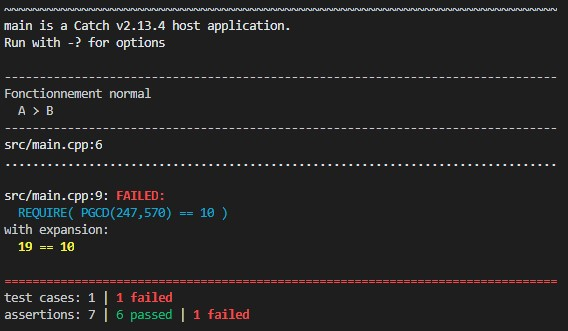
\includegraphics[width=15cm]{Pictures/test_failed.jpg}
            \caption{Exemple d'affichage en cas de test échoué}
            \label{fig:Test_failed}
        \end{figure}

        Dans le cas contraire, on retrouvera l'affichage suivant:
        \begin{figure}
            \centering
            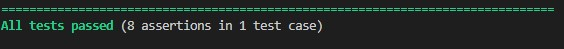
\includegraphics[width=15cm]{Pictures/test_passed.jpg}
            \caption{Exemple d'affichage en cas de test réussi}
            \label{fig:Test_success}
        \end{figure}

        Cepandant, si une erreur ce produit dans une section, cette dernière est abandonée pour passé à la suivante.
        Si d'autre erreurs sont présentes sur d'autre cas de la section, elles ne seront pas visible. Nous n'obtenons pas un rapport total des tests.

\newpage
\section{Hardware}
    \subsection{Etape 1}
        De même que pour l'étape 1 de la partie sotfware, il faut décrire un module VHDL permetant d'implanter le calcul du PGCD de deux nombres.
        Le module aura le prototype suivant :

\begin{lstlisting}[style=VHDL]
ENTITY PGCD IS
PORT ( 
    CLK      : in  STD_LOGIC;
    RESET    : in  STD_LOGIC;

    idata_a  : in  STD_LOGIC_VECTOR (31 downto 0);
    idata_b  : in  STD_LOGIC_VECTOR (31 downto 0);
    idata_en : in  STD_LOGIC;

    odata    : out STD_LOGIC_VECTOR (31 downto 0);
    odata_en : out STD_LOGIC
);
END PGCD;  
\end{lstlisting}
        Le module VHDL fonctionnement grâce à une machine à état.
\begin{figure}[H]
    \centering
    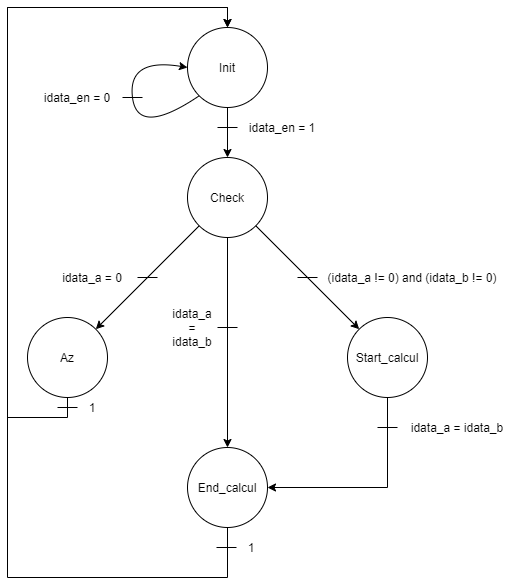
\includegraphics[scale=0.5]{Pictures/FSM_PGCD.png}
    \caption{Machine etat module PGCD}
    \label{fig:FSM_PGCD}
\end{figure}
        La description de cette machine nécéssite 4 process:
        \begin{itemize}
            \item Mise à jour synchrone de l'état
            \item Calcul de nouvelle état en fonction des entrées
            \item Calcul des sorties en fonction de l'état en cours
            \item Cacule du PGCD
        \end{itemize}
    \subsection{Etape 2}
    \subsection{Etape 3}

\section{Conclusion} % Conclusion
\begin{lstlisting}[style=CStyle]
    
\end{lstlisting}

\newpage %-------Saut de Page---------
\listoftodos

\end{document}
